\chapter{Scenario planning tools and report}
\label{sec:covid-pipeline-reports}


1. Intro Unraveling of the epidemic since January: from importation models to intervention model
2. Model description
3. Interaction with public-health decision maker. Usefulness of modeling

\section{Model Parameters from truncated data}

We had access to individual-level data from 1093 patients hospitalized in the canton of Vaud up to April 14, 2020. Of all patients, 41\% (448/1093) were female and 59\% were male (645/1093) with a median age of 70 years (Supplementary Material, SM, Figure~\ref{fig:vdage}). Of all the hospitalized cases, 20\% (214/1093) required use of an Intensive Care Unit (ICU).

\begin{figure}[!htb]
    \centering
    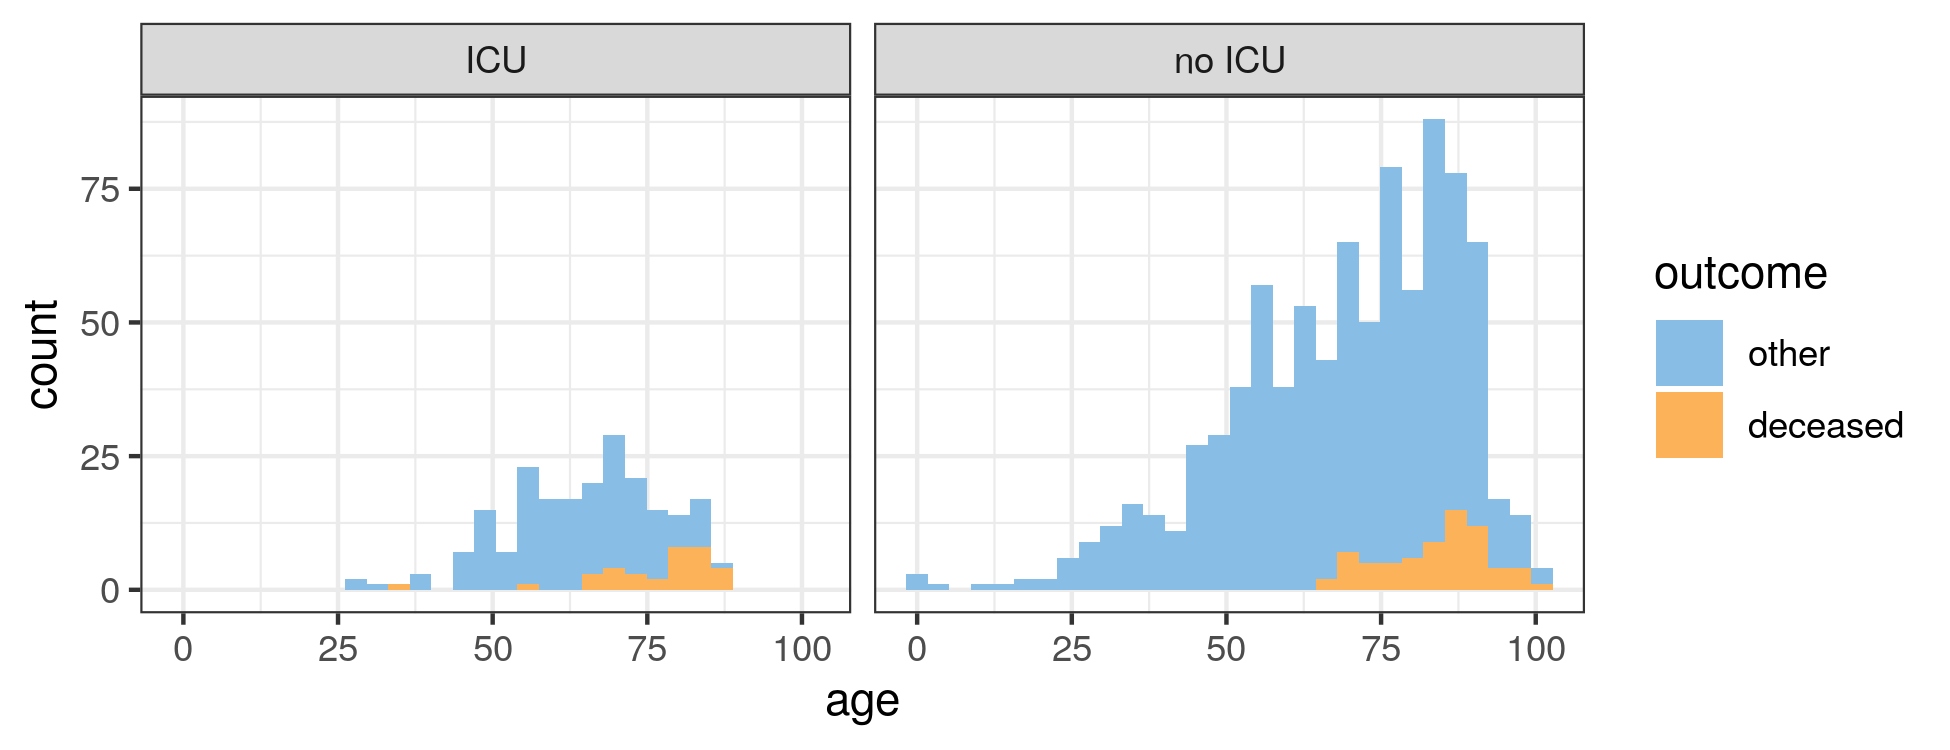
\includegraphics[width = .7\textwidth]{fig_covid-switzerland-npi/fig_supp/VD_hist_age.png}
    \caption{Age distribution of patients hospitalized for COVID-19 in the canton of Vaud up to April 14. Hospitalized individuals are divided in two subgroups depending on if they were treated in ICU (left) or not (right) during their stay. Moreover, only the 777 patients with known outcome are displayed here. We highlight the outcome:  either death (orange) or discharge/transfer to another hospital (blue).}
    \label{fig:vdage}
\end{figure}

Of 777 patients with a known outcome on April 14, 104 died (13\%). 
We estimate the hospitalized Case Fatality Ratio (hCFR) by adjusting for the distribution of time hospitalization to death accounting for the fact that outcomes have not been yet observed for all patients (right-censoring). To account for multiple outcomes (death and discharge), we implement a parametric competing risk survival model similar to that of \cite{Ghani:MethodsEstimatingCase:2005}. We follow a Bayesian approach proposed in \cite{Bellot:TreebasedBayesianMixture:2018} that enables us to fit parametric distributions to times to events using accelerated failure models. This method allows for the joint estimation of the probability of each event type and the distributions of times to events. In this case we are interested in the probability of death, i.e. the hCFR. A COVID-19 modeling study in France identified mixtures of probabilities of times to death, with a group dying faster with exponentially-distributed times and one dying slower \cite{Salje:EstimatingBurdenSARSCoV2:2020}. We therefore extend the Bayesian survival framework to test for mixture in times to death and recovery. We did not take into model patients being discharged from ICU and subsequently dying which was the case for 4/138 patients with known outcome. We neither accounted for multiple ICU stays per patient since we did not have that information. We fit both Gamma and Log-Normal distributions separately to patients that did not go into ICU, and patients that did. For the former, we model times from hospitalization to death or discharge, and for the latter times from ICU entry to both outcomes. Models were fit with Stan \cite{Carpenter:StanProbabilisticProgramming:2017}, and selection was done using Bayesian leave-one-out cross-validation \cite{Vehtari:PracticalBayesianModel:2017}. \\

Times to death and discharge were best described by log-normal distributions with a single group both for patients having required ICU or not (SM Fig.~\ref{fig:delays}). When accounting for right-censoring and assuming log-normally distributed times to events, we estimate an overall hCFR of 16.0\% (95\% credible interval, CrI: 12.5-19.8), resulting from a hCFR of 28.1\% (95\% CrI: 16.4-40.9) for patients requiring ICU and 13.0\% (95\% CrI: 9.9-16.6) for patients that did no require it. Estimated hCFRs were slightly higher when assuming gamma-distributed times to events (overall hCFR of 20.3\%, 95\% CrI: 15.9-24.1).

\begin{figure}[!htb]
    \centering
    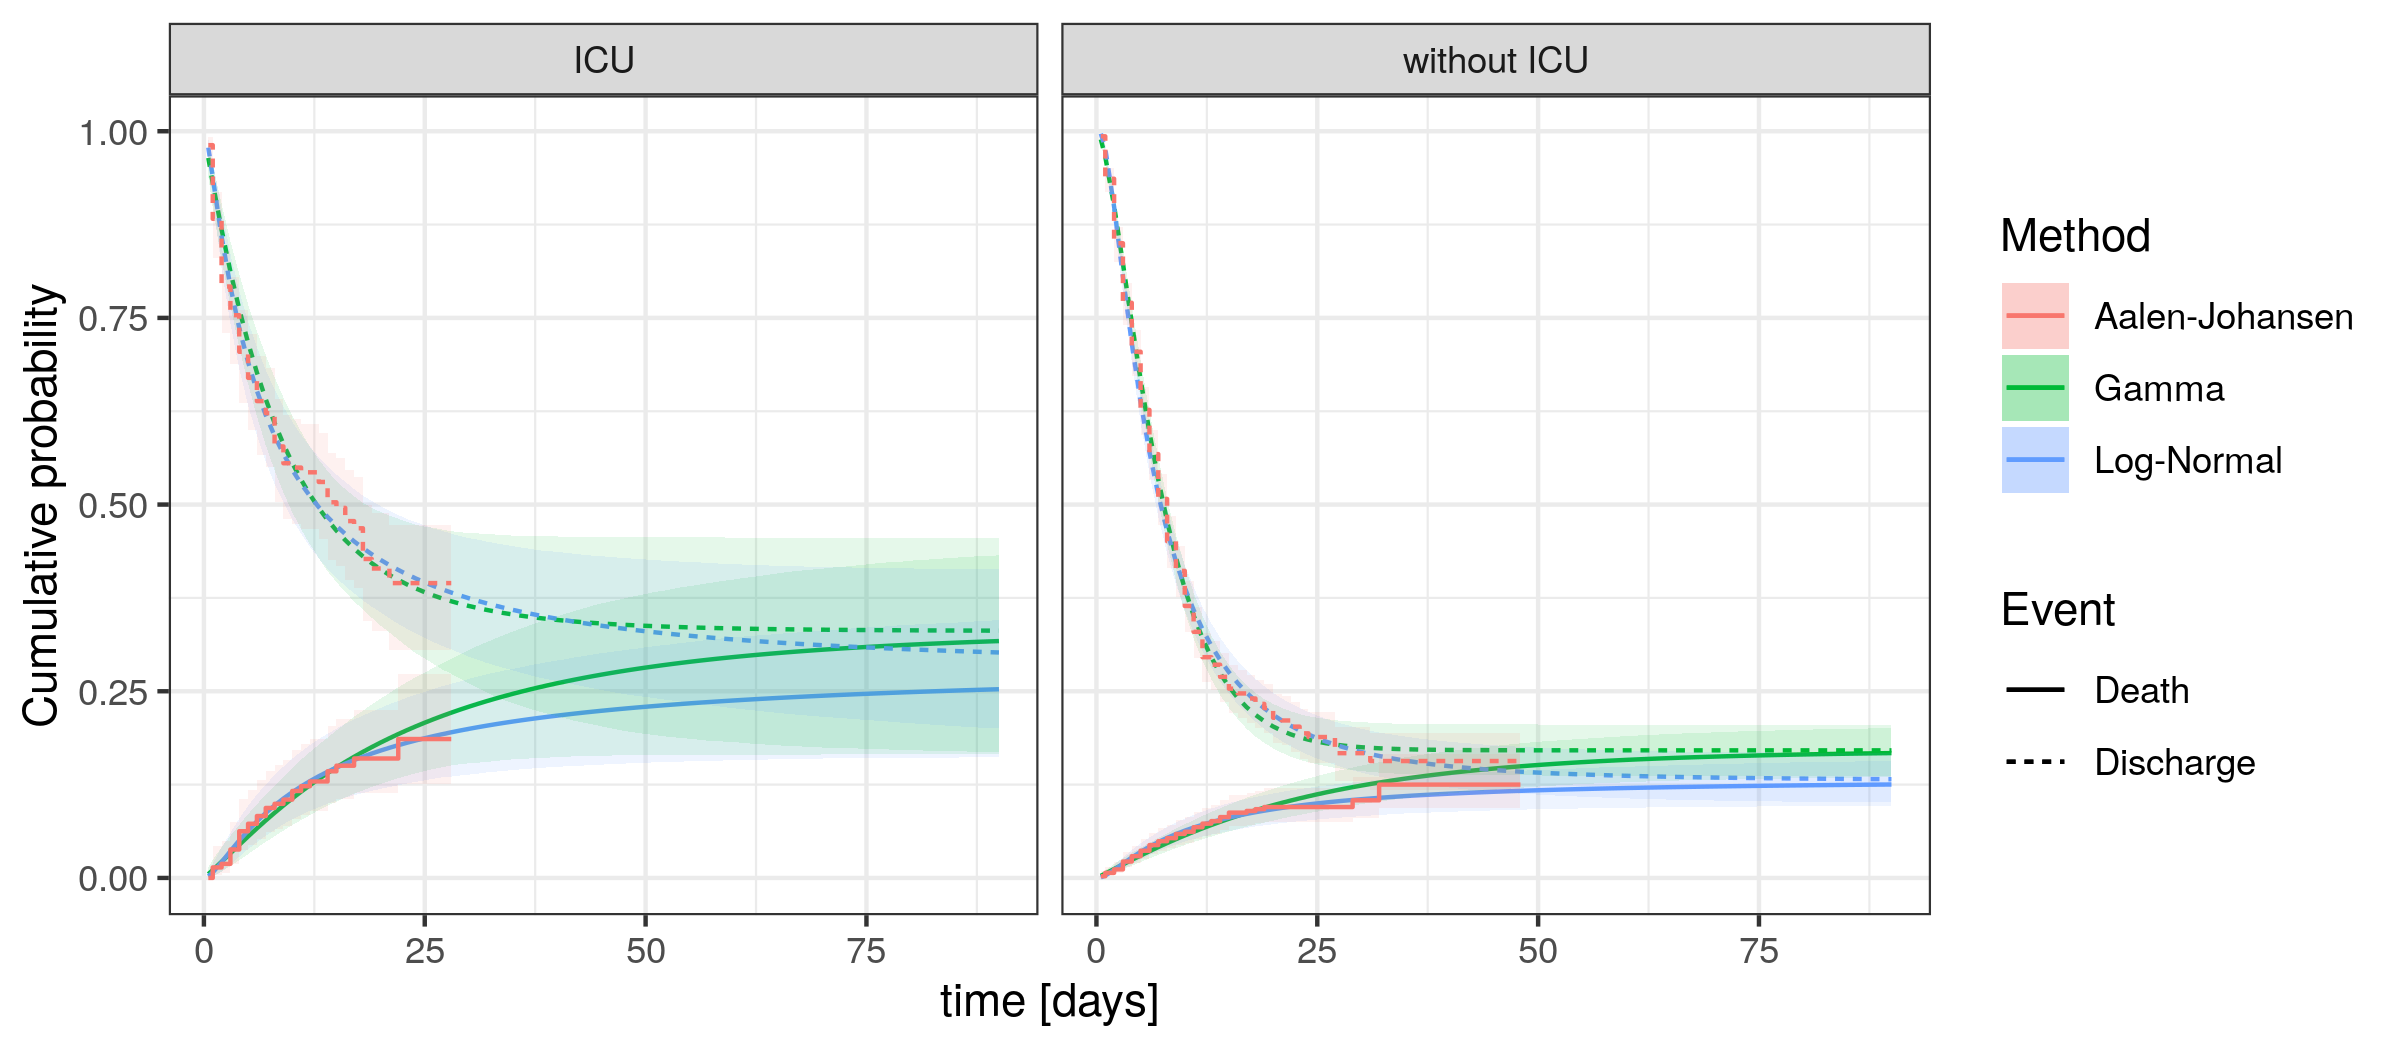
\includegraphics[width=.8\textwidth]{fig_covid-switzerland-npi/fig_supp/survival_analaysis.png}
    \caption{Survival functions of death and discharge for hospitalized patients and patients in ICU. The lines represent the mean estimated cumulative probability of dying (full) and 1 minus the cumulative probability of discharge (dotted) estimated with non-parametric (Aalen-Johansen estimator, shading gives the 95\% CI) and parametric (assuming gamma and log-normal distributions, shading indicate the 95\% CrI) methods. Time is in days from hospitalization for patients that did not require ICU, and time from ICU admission for those that did. The point at which the lines join represents the probability that the final outcome is death, which was estimated to be 28.1\% (95\% CrI: 16.4-40.9) for patients in ICU and 13.0\% (95\% CrI: 9.9-16.6) for patients not requiring ICU based on the log-normal distribution.}
    \label{fig:delays}
\end{figure}

\noindent The distribution of times of hospitalization processes are shown in SM Fig.~\ref{fig:vdtimes}, and fitted distribution parameters given in SM Table~\ref{tab:vdparams}.

\begin{figure}[!htb]
    \centering
    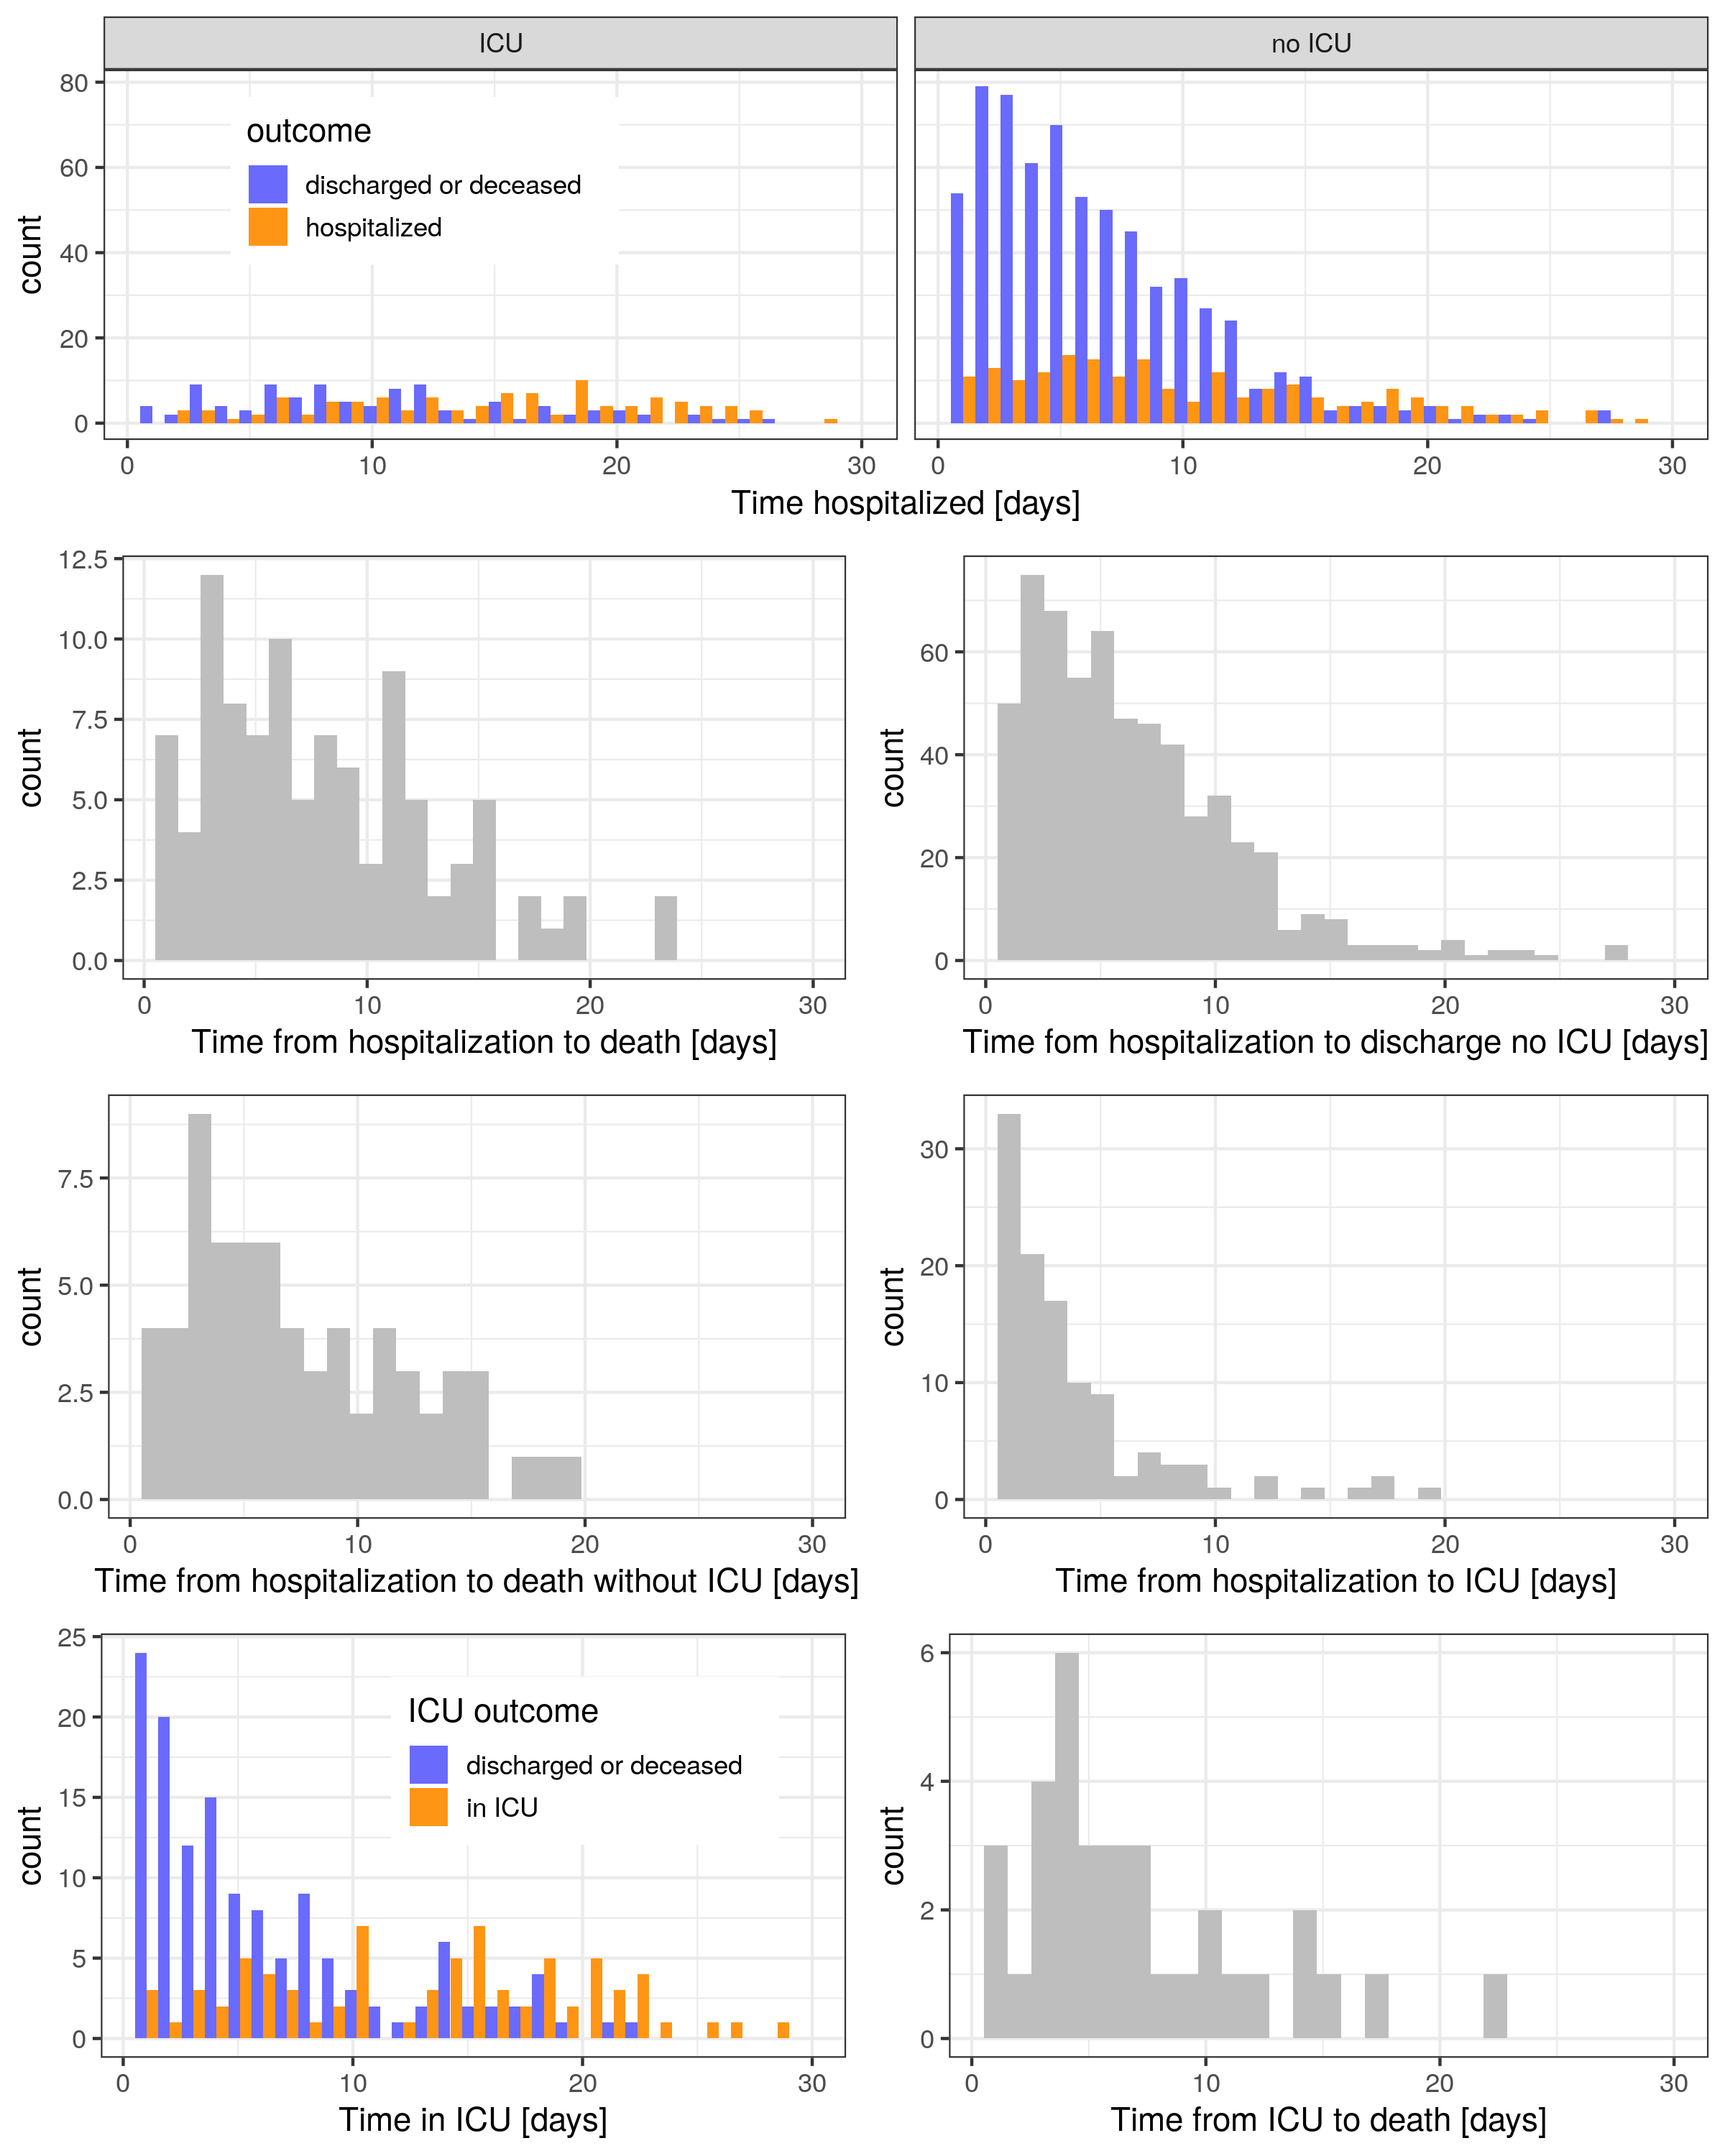
\includegraphics[width=.8\textwidth]{fig_covid-switzerland-npi/fig_supp/VD_times.png}
    \caption{Data from canton de Vaud showing times to key hospitalization events. In order to perform this analysis, we split patients in two categories: those who did not go through ICU during their stay and those who did. From left to right, top to bottom: total length of hospital stay for patients that went to ICU, then similarly for patient that did not. Then we show the time to death for all patients, followed by both the time to discharge and to death for non-ICU patients. The last three graphs concerns ICU patients and detail ICU focused estimate: time from hospitalization to ICU, time in ICU and time from ICU to death. When meaningful, we show both currently hospitalized patient (orange) and already out-of-hospital patients (blue).}
    \label{fig:vdtimes}
\end{figure}

\begin{table}[t]
\caption{Observed hospitalization time distributions. All times are in days and taken from the date of hospitalization if not specified otherwise. Note that these estimates are biased due to right-censoring of observations and probably under-estimate the true distributions. SM Table~\ref{tab:survpars} shows estimates that account for right-censoring.}
\label{tab:vdparams}
\centering
\begin{tabular}{lrrrr}
\toprule
 & mean & sd & mean (logscale) & sd (logscale)\\
\midrule
Time hospitalized & 8.49 & 6.58 & 1.81 & 0.87\\
Time to death & 8.23 & 6.09 & 1.80 & 0.87\\ \addlinespace
Time to discharge without ICU & 6.29 & 4.66 & 1.56 & 0.80\\
Time hospitalized without ICU & 7.35 & 5.79 & 1.68 & 0.85\\
Time to death without ICU & 7.84 & 6.27 & 1.73 & 0.88\\ \addlinespace
Time to ICU & 2.35 & 3.79 & 0.18 & 1.05\\
Time hospitalized with ICU & 13.14 & 7.50 & 2.37 & 0.72\\
Time in ICU & 8.36 & 6.76 & 1.69 & 1.04\\
Time from ICU to discharge & 8.68 & 6.99 & 1.71 & 1.07\\
Time from ICU to death & 6.97 & 4.98 & 1.68 & 0.77\\
\bottomrule
\end{tabular}
\end{table}


\begin{table}
    \centering
    \begin{tabular}{ccccccc}
\toprule
 & & \multicolumn{3}{c}{Log-Normal} & \multicolumn{2}{c}{Gamma}\\ \cmidrule(rl){3-5} \cmidrule(rl){6-7}
Group & Event & median & mean-log & SD-log & scale & shape\\
\midrule
Without ICU & Death & 10 (7.3-16) & 2.3 (2-2.8) & 1.2 (0.95-1.5) & 21 (21-22) & 1.1 (0.83-1.4)\\
 & Discharge & 6.1 (5.6-6.6) & 1.8 (1.7-1.9) & 0.93 (0.87-0.99) & 4.3 (4.4-4.2) & 1.8 (1.6-2)\\ \addlinespace
ICU & Death & 13 (6.2-30) & 2.6 (1.8-3.4) & 1.3 (0.87-1.9) & 21 (12-23) & 1.2 (0.74-1.9)\\
 & Discharge & 6.4 (4.3-9.3) & 1.8 (1.5-2.2) & 1.3 (1.1-1.6) & 9.1 (8.1-11) & 1 (0.75-1.4)\\
\bottomrule
\end{tabular}
\caption{Estimated parameters of hospitalization time distributions. These estimates differ from observed values given in Table~\ref{tab:vdparams} by accounting for right-censoring of observations. We report time from hospitalization to discharge or death, and from ICU admission to discharge or death. Estimates were obtained using competing risk survival model as described in section~\ref{sec:crm}. Parameters are given in terms of their posterior mean and 95\% CrI (in parenthesis). For the log-normal distribution the parameters correspond to the mean and SD of the logarithm of the distribution.}
     \label{tab:survpars}
\end{table}

